%
% Document template suitable for use as a latex master-file for masters
% thesis in University of Turku Department of Information Technology. 
% Relies on itpackage.sty for additional definitions.
%
% Sami Nuuttila (samnuutt@utu.fi) 
%
% Last mod 2.9.2015:
%
%%%%%%%%%%%%%%%%%%%%%%%%%%%%%%%%%%%%%%%%%%%%%%%%%%%%%%%%%%%%%%%%%%%%%%%%%%%
%
% load all required packages
%
%%%%%%%%%%%%%%%%%%%%%%%%%%%%%%%%%%%%%%%%%%%%%%%%%%%%%%%%%%%%%%%%%%%%%%%%%%%

% document is based on report class
\documentclass[a4paper,12pt]{report}

% load ams-packages for maths
\usepackage{amssymb,amsthm,amsmath}

% load url package for urls, specifically in references
% Use hyphenation
\usepackage[hyphens]{url}
\usepackage{hyperref}

% JH: modified latin to UTF-8 encoding cues to make Scandinavian characters works
\usepackage[utf8]{inputenc}
% load babel-package for automatic hyphenation
\usepackage[english]{babel}

\usepackage{ifpdf}
\usepackage{graphicx}

% Allows for full text citations
\usepackage{bibentry}

% load tocbibind package 
%   - do not include table of contents in itself
%   - convert the name of bibliography to references
\usepackage[nottoc]{tocbibind}

% load sverb package
%   - enhanced handling of verbatim stuff; listing environment
\usepackage{sverb}

% load listings package
%   - handle inclusion of source code
% Use listings-rust from ./thesis/listings-rust.sty
\usepackage{listings}
\usepackage{thesis/listings-rust}

\lstset{showstringspaces=false,
  columns=fullflexible,
  escapechar=@,
  basicstyle=\small\sffamily\linespread{0.8},
  commentstyle=\mdseries
}

%\pdfminorversion=7

% load fancyheaders package
%   - the actual headers and footers are set later
\usepackage{fancyhdr}

% load itpackage 
%   - additional defines and stuff
\usepackage{thesis/itpackage}

\usepackage{hyperref}

% \lstset{language=Rust, style=boxed}
% \lstset{basicstyle=\tiny,style=mystyle}

% uncomment the following snippet to get rid of Luku/Chapter text at the
% beginning of each Chapter... 
%\makeatletter
%\renewcommand{\@chapapp}{\relax}
%\renewcommand{\@makechapterhead}[1]{%
%  \vspace*{50\p@}%
%  {\parindent \z@ \raggedright \normalfont
%    \ifnum \c@secnumdepth >\m@ne
%        \huge\bfseries \@chapapp\space \thechapter\space\space
%    \fi
%    \interlinepenalty\@M
%    \Huge \bfseries #1\par\nobreak
%    \vskip 40\p@
%  }}
%\makeatother

\begin{document}

\selectlanguage{english}

% Set some names based on selected language; no modification required
\settocbibname{References}
\renewcommand{\appname}{Appendices}

% Fill in your information below
\workinfo{Jani Anttonen}
{Proof of Latency Using a Verifiable Delay Function}
{Jaakko Järvi}
{Najmul Islam}
{2021}
{May}
{Toukokuu}

% Set the type of your thesis (Diplomityö, TkK -tutkielma, etc.) and
% laboratory or field of study below
\worktype{Master's Thesis}{M.Sc.}
\deptinfo{Department of Future Technologies}

% Generate the title page 
\gentitle

% Include the abstract
% % !TeX root = ../index.tex
\begin{itabstract}{list, of, keywords}
	Tarkempia ohjeita tiivistelmäsivun laadintaan läytyy opiskelijan
	yleisoppaasta, josta alla lyhyt katkelma.
	
	Bibliografisten tietojen jälkeen kirjoitetaan varsinainen tiivistelmä.
	Sen on oletettava, että lukijalla on yleiset tiedot aiheesta.
	Tiivistelmän tulee olla ymmärrettävissä ilman tarvetta perehtyä koko
	tutkielmaan. Se on kirjoitettava täydellisinä virkkeinä,
	väliotsakeluettelona. On käytettävä vakiintuneita termejä. Viittauksia
	ja lainauksia tiivistelmään ei saa sisällyttää, eikä myäskään tietoja
	tai väitteitä, jotka eivät sisälly itse tutkimukseen. Tiivistelmän on
	oltava mahdollisimman ytimekäs n. 120 -- 250 sanan pituinen itsenäinen
	kokonaisuus, joka mahtuu ykkäsvälillä kirjoitettuna vaivatta
	tiivistelmäsivulle. Tiivistelmässä tulisi ilmetä mm.  tutkielman aihe
	tutkimuksen kohde, populaatio, alue ja tarkoitus käytetyt
	tutkimusmenetelmät (mikäli tutkimus on luonteeltaan teoreettinen ja
	tiettyyn kirjalliseen materiaaliin, on mainittava tärkeimmät
	lähdeteokset; mikäli on luonteeltaan empiirinen, on mainittava käytetyt
	metodit) keskeiset tutkimustulokset tulosten perusteella tehdyt
	päätelmät ja toimenpidesuositukset asiasanat
\end{itabstract}
 BROKEN ATM

% empty pagestyle for table of contents etc. 
%
% the redefinition of plain style works also for 1st pages of chapters,
% which is the default in report class. Just state \thispagestyle{empty}
% after \chapter{something} if you want empty style for the 1st pages. 
%
\pagestyle{empty}
\fancypagestyle{plain}{
  \fancyhf{}
  \renewcommand{\headrulewidth}{0 pt}
}

% roman numbering for table of contents etc.
\pagenumbering{roman}

% insert table of contents, list of figures, list of tables
%
% setting the counter to zero effectively removes the page number from
% the toc, lof etc. entries in the toc since there is no roman numeral
% for zero ;-) (if you want them without numbering)
%
%\setcounter{page}{0}
\tableofcontents
\clearpage
\setcounter{page}{0}
\listoffigures
\clearpage
\setcounter{page}{0}
\lstlistoflistings

% possibly insert 'list of acronyms'
%
%   - create a chapter called List Of Acronyms (or whatever), which
%     should contain all your acronym definitions, e.g. 
%     \chapter{List Of Acronyms} 
%   - the secnumdepth trickery is needed because acronyms are as a
%     standard chapter and we are faking '\listofacronyms'
%
%\setcounter{secnumdepth}{-1}
%% !TeX root = ./Terms.tex
\section*{Käsitteet}
\begin{description}
	\item[BASE] \hfill 
			
	\textbf{Basically Available} -- Jokaiseen kyselyyn vastataan, palautusarvolla ei väliä.
	\item[Ebin] \hfill
	ebon 
\end{description}

%\setcounter{secnumdepth}{2}

% setup page numbering, page counter, etc.
\startpages

%%%%%%%%%%%%%%%%%%%%%%%%%%%%%%%%%%%%%%%%%%%%%%%%%%%%%%%%%%%%%%%%%%%%%%%%%%%
%
% Thesis starts here. Create a new tex file for each chapter and input it below. You may encounter errors if you use å, ä, ö or <space> characters in referred names.
%
% Good luck!
%
%%%%%%%%%%%%%%%%%%%%%%%%%%%%%%%%%%%%%%%%%%%%%%%%%%%%%%%%%%%%%%%%%%%%%%%%%%%

% !TeX root = ./Thesis.tex
\chapter{Introduction}
\label{Introduction}

Computer applications, whether they are on the public Internet or on a private network, commonly use the client-server model of communication. In this model, the client application sends requests to the server, and the server responds. Applications are today, however, increasingly moving towards a distributed, peer-to-peer (P2P) networked model, where every peer, whether it is an entire computer or merely a process running on one, serves equally as the both sides of the client-server model. Many uses of P2P are not visible to the end user, because in many cases, P2P technologies serve to optimize resource utilization rather than as centerpoints of applications. For example, the music subscription service Spotify's protocol has been designed to combine server and P2P streaming to decrease the load on Spotify's servers and save bandwith, and thus improve the service's scalability.~\cite{Kreitz_undated-yp} Naturally, P2P streaming comes in handy also whenever there is a short outage, as users might not experience any stoppages to the service, at least when listening to widely streamed content. 

The aspects of peer-to-peer networking that have recently gotten attention are cryptocurrency and blockchain technologies, categorized under the roof term of distributed ledger technologies. Prior to the emergence of ledger technologies, peer-to-peer systems were often seen in the public light as a technology to work around regulations and for doing lawless activities. This is partly because before their use in blockchain applications, P2P systems were popularized for their use in file sharing applications like Bittorrent. Obviously, this reputation was not earned for nothing, but peer-to-peer networking's use in torrents and other file sharing networks also demonstrates its potential in content delivery networks, or CDNs for short. Peer-to-peer networks are not without problems. One persistent source of problems is routing and peer discovery. Since the users of a P2P network do not necessarily connect to a centralized and optimized server infrastructure with vast bandwidth and computation resources, the individual connections between peers can be ephemeral, and routes between peers that are not directly connected are usually random. This results in some routes between peers to be inoptimal, which could result in bad performance and even false states in distributed ledgers, where slow data propagation in a P2P publish-subscribe network could mean inability to participate in the consensus due to latency. % AND THEN WHAT yes, describe the problem

Blockchain networks need a way of synchronizing the latest state of the blockchain globally between a number of peers on a P2P network. Since the blockchain data model is sequential and all recorded history is immutable, an algorithm is needed to reach total synchronization and agreement between peers. This kind of an algorithm is called a consensus algorithm. Consensus problems are not unique to blockchains, but are also relevant in distributed databases. Blockchains have raised new issues in consensus algorithms that have sparked an ongoing development effort for new kinds of consensus algorithms.

Proof of Work is the most used consensus algorithm in public blockchains today, including in Bitcoin, where it was first described in 2008.~\cite{Nakamoto2019-ax} In short, in Proof of Work all participants try to guess a correct answer to a cryptographic puzzle as fast as they can, and a correct answer produces a new block. The new block gets sent and propagated to the network, and if enough peers agree that the answer was correct, the guessing game starts over. In Proof of Work, any latency at all results in wasted resources for all participants before they receive the latest block, as they are still trying to solve the puzzle before they know the result.

As latency is not only a physical and a computational problem in P2P networks, but rather an algorithmic one, search for alrorithmic solutions has long been a part of P2P networks research. Since latency between peers in P2P networks is a problem of the network topology, the solutions have tried to optimize the peer discovery mechanisms. This has worked to some degree, with randomized peer discovery and a high amount of concurrent connections resulting in P2P networks with good peer discoverability and resource availability, but with subpar routes between peers that are not directly connected to each other.

If a peer told you its individual latencies to other peers on its routing table, couldn't this help with constructing an optimal distributed routing table, with peers only connecting to other peers if they are actually close-by or behind a fast connection? I think that it could, but since only a certain number of connections can be kept at one time, this would increase the possibility for so-called eclipse attacks. In an eclipse attack, an attacker tries to influence the victim's connections in a way that it would only be connected to peers controlled by the attacker, effectively isolating the victim from honest peers on the network, increasing the possibility for man-in-the-middle attacks regarding the victim's sent requests or received responses. Also, a not-so-malicious peer could try to game the peer discovery algorithm in the pursuit of better connections to itself at the cost of others. Whilst this is not as severe of a problem, it's still undesirable.

Now, what if you didn't have to trust the peer who reports the latencies, and there was no way for the other peer to lie on the subject? Given this, a peer could roughly estimate the network topology and find the peers closest to it with a roughly optimal amount of queries, and the P2P network could converge towards an optimal topology with limited threat of eclipse attacks. Such a proof of latency could also be used to prove a geographical location, which could be used to battle GPS spoofing. Usually, GPS is a user-facing technology and an individual tool for pathfinding, with only the user requiring the coordinates to be correct so that they won't drive to the wrong cottage. Some applications might require some sort of a proof of a physical location, and this can be done in a centralized manner with bluetooth beacons or with something resembling COVID-19 contact tracing. In a trustless P2P setting, however, this is not as easily achievable without introducing an incentive structure or requiring the use of trusted computation modules.  


% TODO: Elaborate on eclipse attacks, add citations on the matter
Using a verifiable delay function, I propose a novel algorithm for producing a publicly verifiable proof of network latency and difference in computation resources between two participants in a peer-to-peer network. This proof can be used for dynamic routing to achieve better, faster routes between peers, and for making eclipse attacks\footnote{Eclipse attack means polluting the target's routing table restricting the target's access to the rest of the network, which opens up other attack possibilities.} harder to achieve. 


% Background
% !TeX root = ./Thesis.tex
\chapter{Background}
\label{Background}

% !TeX root = ./Thesis.tex
\chapter{Cryptography}
\label{Cryptography}

% TODO: Nobody can understand crypto based on this definition. Start with an explanation that foresees what the chapter will contain.
Modern cryptography is based on relatively few mathematical fundamentals. The most dominant  have historically been prime numbers and modular multiplication, but elliptic curve cryptography is increasingly considered to be the most secure method out there to keep things colloquial.

Modular multiplication with large numbers has a useful property that you can exchange encrypted data without the participants knowing each other's private keys, but requiring a computation that is theoretically almost impossible to break. Prime numbers and elliptic curves can be used to create the variables used in modular multiplication, providing the basis for the robustness of the cryptosystem.
% HAH TÄÄ ON IHAN PASKA ATM, get a grip

\section{Groups of Unknown Order}

\subsection{RSA}
RSA is named after it's discoverers – Rivest, Shamir, Adleman. It is an asymmetric public-key cryptosystem, meaning that it is based on a keypair, in which one is a public and the other is a secret. The public key is used to encrypt, and the secret key is used to decrypt. This means that everyone who has the public key can encrypt data and that encrypted data is practically impossible to decrypt without the secret key. This works due to the fact that it is hard to factor the product of two large prime numbers.

RSA is an arithmetic trick that creates a mathematical object called a trapdoor permutation. Trapdoor permutation is a function that transforms a number x to a number y in the same range, in a way that computing y from x is easy using the public key but computing x from y is practically impossible without knowing the private key. The private key is the trapdoor.\cite{Aumasson2018-nh}
% TODO: Reader thinks what the hell is the next paragraph about, try to open things up a bit before going into factoring competitions, although they play a big part in VDF history

Some institutions also have been publishing these products of two large prime numbers, claiming they have discarded the two prime numbers that were used in the creation. These are published as public puzzles with prizes for correct factorizations as high as 200000 US dollars, but the larger ones can also be used in cryptography to remove a trusted setup. These products are called RSA numbers, of which RSA-1024 and RSA-2048 are widely used. They can be considered relatively safe for production use, since the latest broken RSA number at the time of writing is RSA-250. Still, in practice, the keys could be still stored by the number's creator, requiring trust towards the institutions or individuals who have published them.

\section{Proofs}
Cryptographic proofs are proofs that depend on the trapdoor nature of cryptographic functions. The most well-known proofs, which are not necessarily thought of as such are cryptographic signatures. Given a public key, a computer in posession of its corresponding private key can produce a signature of any given data, implying together with the data that the computer has seen and processed the data.

Proofs can be private or public. A cryptographic proof can be categorized as public, if a verifier can gather all information required to verify the proof from the transcript of the proof itself, and verify the proof to be correct. Now, since classical cryptography is based on the fact that a computation is asymmetric --- being harder to compute the other way around, a cryptographic proof is still probabilistic in nature, and the security of it based on the parameters used.

% !TeX root = ./Thesis.tex
\chapter{Peer-to-Peer Networking}
\label{Peer-to-Peer Networking}
Peer-to-peer networking, P2P in short, means that two or more devices communicate with each other with both serving as a client and a server simultaneously. P2P networks vary in scope a lot. Some networks are global, while some are as small as a couple of devices in a local area network, which is the case in printer sharing and some IoT installations. P2P networks can be standalone or rely on some existing infrastructure, like the internet. The P2P networks that rely on preexisting infrastructure are called overlay networks.

While overlay networks' addressing and routing is usually based on TCP/IP or UDP/IP, they must introduce a separate routing scheme, like a DHT, that works as an index for peers on the network. Since IP only focuses on addressing the computers and not the applications or resources they offer, it can't function as a peer discovery scheme by itself.

Overlay P2P networks must somehow signal the initial peers, also called bootstrap or introductory peers, to connect to at first. This can be done either by including the bootstrap peers' IP addresses in the application code itself or by providing the same information on a regular web page. The bootstrap peers can be also signaled by word-of-mouth between a group of people, or with wireless broadcast, which I will touch a bit on the next section. This said, usually every peer can function as a bootstrap peer, so knowing the connection info of a single peer on the network can potentially introduce you into the network at large.

A simple way to create a P2P network would be to share a single file with anyone who connects to you that has all the IP addresses you've ever connected with. This would be an example of an unstructured P2P network, which could work relatively well in a closed setting, like inside a LAN if there's no support for multicast DNS, or mDNS in short.

\begin{figure}
	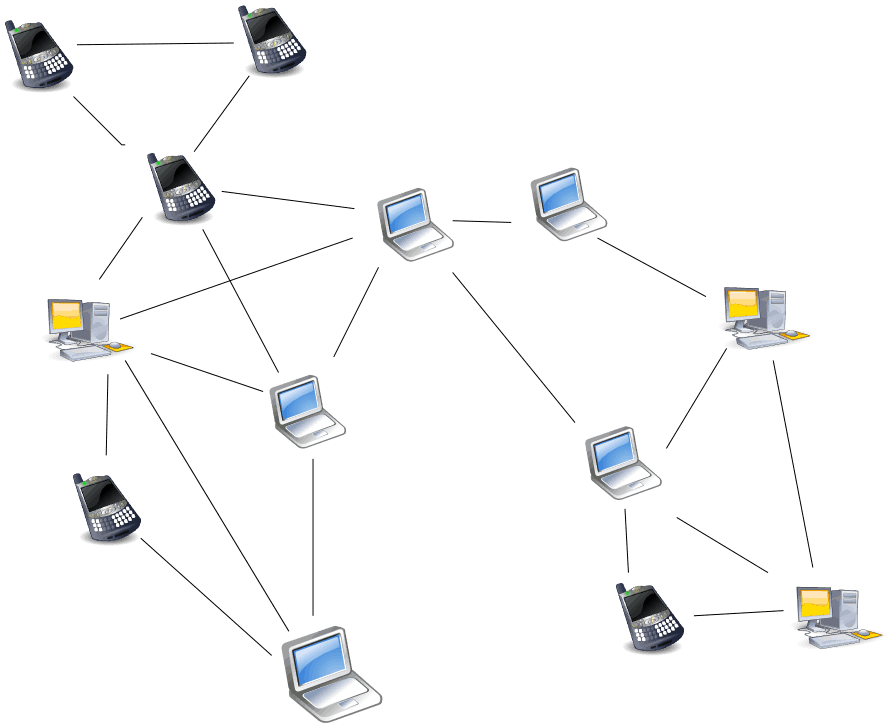
\includegraphics[width=\textwidth]{pictures/unstructured.png}
	\caption{Example topography of an unstructured overlay network}
	\label{Unstructured Overlay Network}
\end{figure}

In contrast to unstructured networks, where peers are connected to at random, structured networks have some logic that is used to form a structured overlay network rather than just connecting to peers as they come.

\begin{figure}
	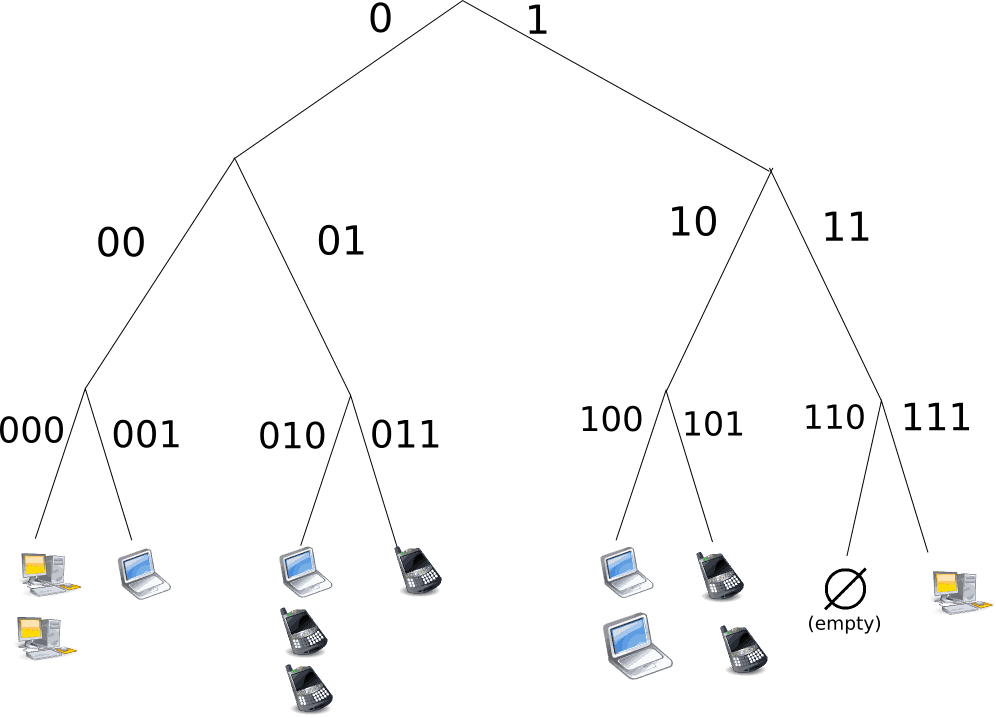
\includegraphics[width=\textwidth]{pictures/structured.png}
	\caption{Example topography of a structured overlay network}
	\label{Structured Overlay Network}
\end{figure}

\section{Ad Hoc and Zero Configuration Networking}
Multicast DNS was proposed by Apple in 2013~\cite{Cheshire2013-ja} as a way of discovering peers in a local area network in a zero-configuration manner. It is used today for resource sharing, such as sharing printers. Multicast DNS does not work outside local area networks, since it works by associating names with IP addresses like regular DNS does. The problem is that these names are not quaranteed to be unique, and therefore can be spoofed. If there are two clients with the same name, the first one to respond with its IP address to a query wins.~\cite{Pdp2008-tg} The security of zero-configuration and ad hoc networking must relay on cryptographic identities, so that a peer can verify itself with public-key cryptography, that makes the peers on the network practically unique and thus hard to spoof.

% TODO: Seuraavaksi väite, cite!
Zero-configuration networking in an unconstrained, global setting is possible with radios, using either dedicated meshnet radios like GoTenna~\cite{GoTenna_undated-km} or Helium~\cite{Helium_undated-jv}, or by using the antennas inside mobile devices to form a network. These types of networks are usually called meshnets or ad hoc networks. Basically, Walkie-Talkies are the simplest form of a P2P network. Problems can arise due to geography blocking signals, or when you want to cross large distances with the transmitting capability of a pocket device. Mesh networking has been used most famously in protests worldwide by using a smartphone app called Firechat.~\cite{Milian2014-mt}

Ad hoc mesh networks have a natural metric for latency, signal strength. They can rely on Bluetooth RSSI\footnote{Received Signal Strength Indication}, or triangulate distances by cooperating with multiple peers. These methods are used to locate emergency calls, and in contact tracing.~\cite{Biddle2020-kl} Mesh networks, while being peer to peer and not relying on existing infrastructure like overlay networks, still need routing and multiple hops if one wants to reach peers that are not in the operating range of the communication method used. Even ad hoc networks could benefit from having a Proof of Latency, although the proofs should be updated way more frequently because of their mobile nature.

\section{Distributed Hash Tables}
Distributed hash tables are a way of pointing content to peers in a distributed network. In addition to indexing content in content-addressed networks like IPFS~\cite{Labs_undated-uw}, they can function as routing tables, and have been developed to remove bottlenecks in peer search. A hash table is a key-value mapping from a to b. What makes them distributed is the fact that the data stored is meant to be distributed between peers, with not a single peer keeping all the available data in its hash table, but relaying queries for resources it does not have to other peers on the network. There are multiple versions of DHTs with different methods for prioritizing certain peers, using tree structures, sorting by identifiers, using computational trust et cetera.

In addition to identifier closeness, DHTs can force a certain network behavior by peer scoring and constructing a web of trust. For example, a peer could only advertise peers that have been connected over a period of time, or enforce reconnecting to disconnected peers that have a good reputation. Computational trust is bayesian in nature, optimizing a single value over time, and simulating remembrance and forgettance. A widely used trust system like this is TrustGuard, implemented in the blockchain framework Tendermint.~\cite{Srivatsa2005-ib, Jeff_Foley2018-zt}

Most of the DHT algorithms were invented in the early 2000s, with Kademlia being one of them. DHTs mostly differ just by how distance is defined, and how the neighbors are chosen.~\cite{Cai2015-ra}

\subsection{Kademlia}
Kademlia is a DHT designed by Petar Maymounkov and David Mazières in 2002. It is based on a tree of identifiers which are split across peers on a network. The identifiers are 160 bits, e.g. a SHA-1 hash of some larger data. Kademlia tries to improve upon previous DHT-based routing algorithms by introducing a symmetric XOR metric for distance between node IDs in the key space.~\cite{Petar_Maymounkov2020-sx} These IDs are sorted in a binary search tree, with each node's position determined by the shortest unique prefix of its ID, like shown in diagram \ref{Structured Overlay Network} on page \pageref{Structured Overlay Network}. Kademlia makes sure that any node in the network can locate any other node by its ID by making sure that each node knows at least one of the nodes in each subtree.

A single query in Kademlia has been shown in real-world tests to result in an average of 3 network hops, meaning that the query gets relayed through two peers before reaching the requested resource.~\cite{Roos2013-mb} Network hops are a necessary evil in distributed systems, and Kademlia does well in requiring on average a log(n) queries in a network of n nodes. Since the closeness metric is based on a similarity search rather than a measurement, the closest peer is only closest by the identifier, not by network latency.~\cite{Eigenmann2020-zm}

The randomness of Kademlia is great at averaging the network hops required to reach a scarce resource. The downside is that it also averages everything else, increasing latency to closest connected peers, reducing overall performance of the network.

Kademlia protocol has four remote procedure calls, or RPCs in short. These are PING, STORE, FIND\_NODE, and FIND\_VALUE. A Kademlia participant's most important operation is node lookup, which is locating k closest nodes to a given node ID. It is a recursive operation, which starts by picking alpha closest nodes from its closest non-empty bucket, and sending them all FIND\_NODE calls. This is repeated until the initiator has queried and got responses from all k closest nodes it has seen.

\section{Eclipse Attacks}
Although Kademlia is most widely used with random hashed identifiers, the distance metric stays the same. By forging identities that are close-by, you can advertise false friends which take over the search space. For example, in a 2019 paper "Eclipsing Ethereum Peers with False Friends" by S. Henningsen, D. Teunis, M. Florian, and B. Scheuermann, they demonstrate that to eclipse a victim in Ethereum P2P network, you need to fill its 8 slots for outbound connections, and fill 17 slots for inbound connections to completely deny service without going through the attacker's nodes.~\cite{Henningsen2019-mf}

Less structured, random ways of forming connections in an overlay network, like Kademlia, protect against eclipse attacks quite well because of the high connectivity and low locality. Introducing peer scoring and making the network topology more structured opens up possibilities for an attacker to game the scoring system, making sure the target connects to lots of sybil peers eclipsing it. Thus, protecting against eclipse attacks is a balancing act that requires an overlay network to retain some elements of an unstructured network while improving general performance with a structured group of peers.~\cite{Mao2020-ee} This balancing act is seen as a multi-armed bandit problem of exploration and exploitation in the 2020 paper "Perigee: Efficient Peer-to-Peer Network Design for Blockchains" by Y. Mao, S. Deb, S.B. Venkatakrishnan, S. Kannan, and K. Srinivasan.


% TODO: More stuff here

\section{Distance Bounding Protocols}

Distance bounding protocols are interactive protocols that aim to measure the physical distance or latency between two participants, the prover and the verifier. They are solutions to problems where a simple ping will not suffice, as either party could quite easily craft a false measurement. Distance bounding is used in applications like IP geolocation, wireless access control, and routing in P2P (ad-hoc) networks.

The first distance bounding protocol was designed by Brands and Chaum in 1993 to counter so-called relay attacks.~\cite{Boureanu_undated-bn, Brands1994-hz} A commonly used example of a relay attack is that if the signals between a credit or a debit card and a point of sale system were to be relayed over a distance, two attackers could pay with the relayed info in a totally different country, for example. A distance bounding protocol is safe if information never gets passed faster than the speed of light, and if causality holds due to the prover not able to create a valid response to a challenge before it has received it.~\cite{Boureanu_undated-bn}

The original definition of a distance bounding protocol consisted of three phases: initial phase, critical phase, and a verification phase.~\cite{Brands1994-hz, Mauw2018-uz} During the initial phase the two peers agree on the parameters used. After that, the critical phase is executed, where the two peers do multiple challenge/response rounds. The final phase, the verification phase, is optional, because the verifier can also verify the proofs during the critical phase.

A way to infer physical distance \(d\) from the measured round trip time \(\Delta t\) is to convert the latency to an approximation of the round trip time \(\Delta t\) divided by two times two-thirds the speed of light \(c\)~\footnote{an approximation of network transmission speed in optic fiber widely used in IP geolocation~\cite{Candela2020-am}}:

\begin{equation*}
  d = \frac{1}{2}\Delta t \frac{2}{3}c
\end{equation*}

Even when not using distance bounding for geolocation one can use the aforementioned method to pick sane parameters for each application, like attack prevention in point of sale systems and RFID lock tags. For the measurement to be as close to ground truth as possible, there needs to be sufficient computing power and a good software implementation to minimize any processing delay introduced between receiving a challenge and sending the response, as this delay lowers the maximum measured resolution achieved by the protocol. For point of sale systems, this delay can be crucial, as we only want the point of sale system to be used by the customer next to it.

When distance bounding is used in other ways than highly local applications like car keys, e.g. in digital rights management, it can reveal too much of the user's location. Usually distance bounding protocols have assumed that both the prover and the verifier are willing to disclose their locations. Some newer protocols have tried to introduce a cloaking region by reducing measurement resolution by adding a delay to the challenge responses.~\cite{Molina-Martinez2018-nw} This is a welcome solution in instances where a verifier only needs to know a rough estimate of the prover's location instead of a tight bound, for example in content delivery networks.

\subsection{Attacks}
As distance bounding protocols were originally made to solve the problem of relay attacks, they are usually not an issue. That said, most RFID implementations do not use distance bounding protocols to require a maximum distance to the tag, and are vulnerable to so called mafia attacks.~\cite{Nikov_undated-vv}
% !TeX root = ./Thesis.tex
\chapter{Verifiable Delay Functions}
\label{Verifiable Delay Functions}

% TODO: Reduce vagueness, more oomph
A verifiable delay function is a function that calculates sequential calculations that cannot be significantly sped up by parallellisation or skipped, and creates a proof of the calculations that is faster to verify than the calculations are to fully re-evaluate. The computation of a VDF can be split into three distinct parts: Evaluation, proof generation, and verification. The evaluation is the hard sequential calculation from which a proof is generated.  

The common parameters in VDF calculation are random input x, it's hash which is called the generator, the group G, and the amount of sequential operations, also called the difficulty, T.

Verifiable delay functions are a peculiar bunch of cryptographic proofs, since they are not proving that something has happened or something has been seen, but that a certain amount of time has been spent to compute the result. Like other cryptographic proofs, for the proof to be publicly verifiable it must at least in part be based on public parameters. If a VDF is going to be calculated between two parties, these parties decide the starting parameters between themselves, in a way giving the parameters to each other. This is to prevent possible precomputation --- meaning that the peer that provides a VDF proof could have computed it earlier, separately from the current transaction. If a participant or participants can decide the parameters of the computation by themselves, there's no restriction for how far back the computation has occurred.

There's no known way to reduce computation costs sublinearly to the bit length of the exponent used.~\cite{Boneh2018-sm} This means that there's no algorithm-based solution to make VDF computation faster that is not related to other factors like efficiency. Despite this, there is a growing effort in developing faster hardware for VDF evaluation, especially for doing repeated modular squarings, which would speed up both the evaluation and the proof phases of a VDF. 
% This is a bit abrupt, add info on the different requirements of different parts of VDF calculation

\section{Background}
While proof of work is the most widely used consensus algorithm in public distributed ledgers, its use can result in wasteful use of computation resources, especially when there's significant latency between the participating peers. While many other consensus algorithms have been proposed and even applied to distributed ledgers, they come with their own set of problems to tackle. In Proof of Stake network nodes participate in the voting of new blocks by staking a part of their assets as a pawn. Concretely this means that a peer hands the control of some of its cryptocurrency to the consensus algorithm. If a voter gets labeled as malicious, faulty, or absent by a certain majority, its stake can get slashed, losing all or a part of the staked asset in the process. This serves as an incentive for honest co-operation, with sufficient computation resources.

One problem with Proof of Stake is that the block generation votes are not done globally, but by a selected group of peers called the validators, which vote for the contents of proposed blocks that are generated by just one peer at a time, selected as the block generator. The validators are usually selected randomly. This has generated an increasing demand for verifiable public randomness that is pre-image resistant, meaning the output of the algorithm generating the randomness cannot be influenced before evaluation by input. This created a need for an algorithm that would prevent multiple malicious actors from being selected to vote at once. Verifiable delay functions can help in creation of public randomness simply because they produce quickly verifiable proofs for results that have high entropy due to repeated calculations with a pre-image resistant hash function. The hash function inside a VDF can be changed, and VDFs' use in such distributed random beacons is only a small piece of a larger puzzle, as good randomness is hard to achieve using only pseudo-random hash functions. Another problem which served as a motivation to find such a function is scalability and data integrity in distributed ledgers. If the participants of a distributed network of nodes have the same initial input for a high-frequency hash function, and they have similar hardware, it can help putting transactions in order without explicit communication between peers, since you can index each transaction with a hash before communicating it to other peers. The resulting order can be incorrect, but like the case with other forms of synchronized distributed clocks, the main objective is to have an explicit order without ambiguity. This also ties into CRDTs\footnote{Conflict-free Replicated Data Type}, but since that is not the main subject of the thesis, I will not address it.

Time-lock puzzles are precursors to VDFs. Their evaluation can be similar or even identical, but they do not contain a proof that is faster to calculate than to re-evaluate the whole puzzle. One example of such proof would be to link each iteration of the puzzle's evaluation to the previous iteration, and supply each step of the calculation to the proof's verifier. Then the verifier can use parallel computation to verify the proof faster than re-evaluating the whole thing. A proof of this sort is categorized as being a proto-VDF, since there are better and more bandwidth-efficient ways to construct a VDF proof, and some could argue the proof is not strictly a calculated one.

In 2018, two research papers were released independently with descriptions of VDF candidates.~\cite{Wesolowski2018-rf, Pietrzak2018-xs} But before that, also in 2018, a paper formalizing VDFs was published by Boneh, Bonneau, Bünz, and Fisch, mentioning the term for the first time. VDF is an algorithm that requires a specified number of sequential steps to evaluate, but produces a proof that can be efficiently and publicly verified.~\cite{Boneh_undated-ml} To achieve pre-image resistance, meaning that the soundness holds even for an adversial peer with lots of precomputation, a VDF is sequential in nature, and its evaluation cannot be sped up by parallel processing. There are multiple formulations of a VDF, and not all even have a generated proof, instead using parallel processing with graphics processors to check that the delay function has been calculated correctly.~\cite{Yakovenko2018-zn} This bars less powerful devices, like embedded devices, from verifying the VDF's result efficiently. Thus, generating a proof that requires little time to verify is more ideal.~\cite{Boneh_undated-ml}

VDFs could see usage in many things not directly related to blockchains or distributed ledger technologies, and my motivation for this thesis is to find such new use cases. I believe I have found one that is somewhat related to the distributed synchronized clock mentioned earlier, using a similar parallel construct between two peers to measure latency with iterations of a sequential computation.


%TODO add an intro on VDFs from the boneh paper
\section{History}
Verifiable delay functions are based on time-lock puzzles. Like VDF's, time-lock puzzles are computational sequential puzzles that require a certain amount of time to solve.\cite{Rivest_undated-qr} Time-lock puzzles were originally created to encrypt information in a manner that could only be opened after a certain amount of computation. Functionally, this is a cryptographic time capsule. Ronald L. Rivest, Adi Shamir, and David A. Wagner classify time-lock puzzles generally under the term timed-release crypto in their 1996 paper.~\cite{Rivest_undated-qr} They describe the envisioned use cases for timed-release crypto as being the following, and they're very similar with the general concept of sending information into the future:

\begin{itemize}
	\item A bidder in an auction wants to seal his bid so that it can only be opened after the bidding period is closed 
	\item A homeowner wants to give his mortgage holder a series of encrypted mortgage payments. These might be encrypted digital cash with different decryption dates so that one payment becomes decryptable and thus usable by the bank at the beginning of each successive month
	\item An individual wants to encrypt his diaries so that they are only decryptable after fifty years.
	\item A key escrow scheme can be based on timed-release crypto so that the government can get the message keys but only after a fixed period, say one year
\end{itemize}

Verifiable delay functions fall under the same category, but introduce a publicly verifiable proof that is much faster to verify than the puzzle was to solve. The original motivation for verifiable delay functions was to enable someone to pick off where somebody else had left when calculating a time puzzle --- to make it possible to create checkpoints in the calculation that could be trusted. Around the same time, VDFs found use in blockchain applications as a way to achieve unspoofable randomness in elections and smart contract input.

% TODO: Proofs of Sequential Work or PoSW

\section{Variations}
There are multiple variations on the security principles used, since a VDF can use any group of unknown order as a basis for its unpredictability. Known solutions use RSA, elliptic curves and class groups as their cryptographic basis.

% TODO ADD MATH, DEFINITIONS, Explain how VDF works!

Since I am using the Wesolowski proof in Proof of Latency, I will concentrate on it the most here, but will also explain differences between the most known ones. For the group of unknown order I will use the RSA group in the examples.

\subsection{Wesolowski's Efficient Verifiable Delay Function}
The "Efficient" in the name of this VDF protocol by Benjamin Wesolowski means that the proof it generates is efficient to verify by a third party, in this case \( \log _{2} T \) multiplications, with \( T \) being the total amount of modular multiplications proven. The following is a description of the non-interactive\footnote{Requiring no messages to be sent --- no interaction} variant of the protocol and its phases.

\( let \: N = RSA-2048, \mathbb{G} \; = \: multiplicative \: group \: of \: integers \: modulo \: N \)

\( let \: x \: = random \: input,  \: H \: = hash \: function, \text{for example} \: BLAKE3 \)

\( let \: generator \: g = H(x) \to \mathbb{G}, T = difficulty \)
\begin{enumerate}
	\item{Evaluation}
																	
	To evaluate the VDF, one must calculate T repeated modular squarings. This means raising the generator $g$ to the power of 2 and taking the remainder of that result divided by $N$, $T$ times.
																	
	As an equation the evaluation output is the following:
																	
	\( output = g^{2^{T} \mod N } \) 
																	
	\item{Proof Generation}
																	
	\( let \: L = random \: prime \: number \)
																	
	\( let \: q \in \mathbb{Z}, q = 2^T/L, \: \text{(quotient)} \)
																	
	\( let \: r \in \mathbb{Z}, r = 2^T\mod L, \: \text{(remainder)} \)
																	
	\( let \: proof = g^q \) 
																	
	Now that the proof has been calculated, a verifier needs $N$, $output$, $g$, $L$, $r$ and $proof$ to verify that the proof is correct and the prover has actually calculated $g^{2^{T} \mod N }$.
																	
	\item{Verification}
																	
	To be sure that the prover has calculated the output correctly, a verifier must check the following equation:
																	
	\( output = proof^L * g^r \:, where \: r = 2^T \mod L \)
																	
	If the two sides are equal, the VDF has been verified as being correct!
\end{enumerate}

Different VDF constructs, like the most well known ones, Wesolowski and Pietrzak, make computational trade offs on different parts of the proof. In a Wesolowski VDF the proof generation is a significant part of the whole VDF calculation, comparable in time to the evaluation itself unless optimized in any way. A Pietrzak VDF is faster to prove, but a lot slower to verify. A Wesolowski VDF produces a proof that can be verified in O(1) time.

In the Proof of Latency chapter under the section Proof of Concept I will demonstrate the Wesolowski VDF as a computer program, programmed in Rust.

% TODO: NOT DONE YET

\section{Similar Constructs}
\subsection{Proto-VDF}
A VDF can only be calculated sequentially, but even without a proof there is a possibility to make the verification faster through parallellism. A non-verifiable delay function, or time-lock puzzle in short, can be still verified faster than the calculation, because there is no sequential requirement after the puzzle has been calculated, enabling to use multiple CPU cores or highly parallel graphics processing units for verifying the puzzle, like in Solana.~\cite{Yakovenko2018-zn} One could also argue that all blockchains and some random beacons form multi-party calculated VDFs. An algorithm based on sequential hashings, like sha-256 in Solana's Proof of History can be described as a proto-VDF, since it can be verified as correct faster than it can be evaluated with hardware, but doesn't have a separate proof.

\subsection{Classic Slow Functions}
Since a VDF's idea is that a hard calculation can be verified faster than to be evaluated, any calculation of which inverse is harder is a candidate for a VDF-type construct. One example of these asymmetric calculations is Sloth.~\cite{Boneh2018-sm} Sloth doesn't include a proof and is not asymptotically verifiable, thus not filling the definition of a VDF per se.\footnote{Asymptotic, meaning that there is a maximum verification time and the verification can't scale beyond that point.} The evaluation of Sloth is calculated with repeated cubic roots, and is verified with repeated cubings, with cubic roots being harder to compute than the cubings.

\section{Use Cases}
Many have shown that there are more use cases for verifiable delay functions than puzzles and random number generators. Some examples include preventing front running in P2P cryptocurrency exchanges, spam prevention and rate limiting.~\cite{noauthor_undated-hk} Almost all use cases are based on the property that with a new unique input, and a difficulty requirement, there is no easy way to speed up the calculation.

In the front-running use case, this property can be used to restrict front-running in both centralized and decentralized exchanges.~\cite{Khalil2019-sl} Front-running is a term used in both stock trading and cryptocurrency trading which means using inside knowledge, or just a faster connection, of a future transaction to trade the asset with a better price or deny the other transaction from happening.~\cite{Robinson2020-ve} The issue is pronounced in trustless P2P networks like the Ethereum blockchain, where pending transactions are for all to see and can be overtook by promising the network validators a bigger reward, since there's no synchronization before consensus is achieved.~\cite{Mitchell2020-hn} In a centralized exchange, preventing front-running with a VDF means that the exchange waits for a specified time before it starts the fulfilling the trade. The VDF serves as a receipt for the order taker that there was no reordering and the take orders were processed in a FIFO\footnote{First in, first out} fashion.~\cite{Cline2020-wb} In a decentralized exchange the same holds, if there exists only one peer that can fulfill the order. The peer then functions exactly like the centralized exchange mentioned before.

Spam prevention and rate limiting in the context of VDFs mean roughly the same thing. This is because spam prevention with VDFs is done with rate limiting. If a network application requires peers to perform some sort of Proof-of-Work in a form of a VDF, by defining the difficulty parameter T they can set a time boundary for subsequent requests, also called a rate limit. If all the peers need to perform a challenge to request resources from the requestee, a performance-based limit is created for the time between each individual request, thus limiting spam. In similar fashion, the deterministic nature of VDFs can be used to make more power-efficient proof-of-work algorithms, by changing the requirement from finding a solution to a random challenge to a predetermined challenge with an exact number of steps. This results in better power efficiency, because it cannot be sped up with parallellism, thus limiting the use of power hungry GPUs or highly parallel ASIC chips for the job.

% TODO: Why the original motivation was left out? Mention Chia's Proof of Space Time, Solana etc PoS type stuff

\section{Hardware Developments}
VDF applications can be made faster with hardware, and it has been estimated that with an ASIC\footnote{Application-Specific Integrated Circuit. A purpose-built chip for a single algorithm.} chip a VDF can be evaluated more than ten times faster than with a GPU.~\cite{Stanford_Video2020-ap}
The three different parts of a VDF calculation are different in terms of the hardware that can be utilized to make them faster. The evaluation part currently has no de facto hardware to make it faster, but the ASIC and FPGA developments are the ones pushing this part forward. Proving can be made faster with GPUs, whilst verification benefits from fast general computation, thus CPUs.\cite{Protocol_Labs_Kelly_Olson2020-au} The chip developments for evaluation also help calculation of zero-knowledge proofs, since they also use repeated squarings for proof generation, thus benefiting cryptography at large.

If or when hardware specifically optimized for sequential squarings is commercialized, VDFs can become much more mainstream, and suffer less from computational differences, thus requiring less trust between the calculating parties. It's a race against time, since if an attacker put a considerable amount of resources in the development of such a chip themselves, they could potentially compromise the security of some blockchains, due to an assumption that's made generally in all blockchains: When competing chains are proposed as the truth, the one with the most work is regarded as the winner. By creating blocks faster than the majority of the network, one could attack proof of stake systems relying on this assumption with a proprietary chip.

Besides the development of an ASIC driven by vdfresearch.org~\cite{noauthor_undated-hk}, there's been development on CPU instructions by Intel, aiming to help the specific operation of modular exponentiation, which is used not only in VDFs, but also in classical RSA, DSA\footnote{Digital signature algorithm}, and DH\footnote{Diffie-Hellman key exchange} algorithms, not to mention homomorphic encryption\footnote{Homomorphically encrypted data is data that can be done calculations with without revealing it's contents to the calculator.}.~\cite{Drucker2019-cx} 



% Design
% !TeX root = ../Thesis.tex
\chapter{Proof of Latency}
\label{Proof of Latency}
Proof of Latency, "the algorithm" or "PoL", is an algorithm that when used in a P2P context, can offer a robust way of reducing network latency between peers by minimizing the number of hops between peers that are close in terms of performance and geographical location. PoL also makes network bootstrapping faster, making it easier to find performant, close-by peers on first interaction with PoL-enabled network. PoL can result in a network in which a peer can estimate its latency to another peer before connecting to it.

The algorithm is trustless and requires no specific hardware from the participants, while a trusted computing platform would make it fairer and more reliable by not discriminating based on processing performance. An ASIC VDF chip would also make any of the later mentioned attack vectors less relevant by removing variance in hardware.

\section{Use Cases}
The section Peer-to-peer Networking described the problems Proof of Latency is trying to solve. While the use in P2P routing might be a no-brainer, the same algorithm can be used for computation performance benchmarking. In the next sections I will describe these use cases more thoroughly.

\subsection{Dynamic P2P Routing}
The use case that drove me to proceed working on Proof of Latency is an idea that there could be a trustless way of telling to other peers how much latency you have to another peer. In current P2P systems, if one peer were to tell you that it had a 10ms latency to another peer, there would be no quarantees of the 10ms latency holding true. If we could make a proof of that latency using cryptography, you could tell that the reported latency is true, and some work has been done to calculate it. This kind of proof could also make eclipse attacks harder to accomplish by requiring a closer distance or more resources to reach a lower latency to the targeted peer.

% TODO: Explain this idea WAAAAAY further

Although DHTs like Kademlia do peer distribution basically at random based on identifier closeness, there are no guarantees that when a peer connects to peers it has received from an another peer are also random, and thus the promise of random peer walk is lost. With Proof of Latency, you can be sure that the peers advertised are actually close-by. Of course, this is easily avoided by the attacker by spawning multiple peers in the same location.

\subsection{Benchmark Queries}
A protocol like this could be used to query for performance. In fact, Proof of Latency does that already, but processor development might render that property less effective in the future, unless one were to measure parallel processing capability with multiple VDFs, for example. Parallel multiple VDFs have been thought of and tested before, but calculating multiple separate VDFs has not been useful in previously imagined use cases, since it doesn't serve as a measure of time, but performance.

This could serve as a part of a greater protocol in a distributed computation system. It would be very unfortunate to run large datasets against a data analysis model on a mobile phone, and it could be beneficial to prove that the peer that advertises its services can actually run the computation without hiccups.
% TODO Cite?
There have been proposals for a VDF-as-a-function system, in which less performant peers could query for a VDF calculation if they don't have the means to do so in a time frame small enough themselves. The FPGA based system is being tested right now on Amazon Web Services cloud platform.~\{Devlin2020-qw} A benchmark query using PoL could also be a part of such a system to verify peers' ability to perform VDF calculations faster than the querying peer.

\section{Role of Latency in Distributed Systems}
It's hardly a surprise, but latency is a huge factor in distributed systems, especially trustless, decentralized ones. Latency is mostly constrained by the speed of light, which can not be changed, and thus there are concrete factors that must be taken into account when designing a P2P system with routing. In 2012, the global average round-trip delay time to Google's servers was around 100ms.~\cite{Grigorik_undated-mc}

In the new space age the maximum possible latency grows very fast, as there could be peers joining to a distributed network from other planets, space ships or stations. This might be unnecessary to think about in the distributed P2P context for now, but before all that, we have global satellite mesh internet providers, like Starlink. Elon Musk, the founder of SpaceX, which provides the network of satellites, claims that there's going to be a round-trip\footnote{Including the user's initial request and received response} latency of about 20 milliseconds between a single satellite and the user.~\cite{Tung_undated-ny} In legacy satellite internet access, the round-trip time even in perfect conditions is about 550 milliseconds.~\cite{noauthor_undated-zc} This difference between legacy and newer satellite internet comes from the difference in their orbits and the sheer amount of satellites involved. Legacy satellite internet uses geostationary orbits, which are very high, beaming on a single face of the earth at a time with limited bandwidth. Newer systems, like Starlink, use a low-earth-orbit, which requires more satellites, since they zoom by at such a speed that constantly changing which satellite you're connected to is a must. The low orbit also means less distance between the satellites and the user. The 20 millisecond latency claimed by Starlink at first seems like a stretch, but is believable when you take into account that inter-satellite links are done by laser, and light can travel about 31 percent faster in a vacuum than in fiber optics.~\cite{Finley2013-wt} Intercontinental latencies can become much lower because of this.
In blockchains, latency plays a role in the efficiency of the power used to achieve consensus. Miners waste energy on a previous block as long as they don't receive information on the winner of the previous block race. Simulations by Wei Bi, Huawei Yang, and Maolin Zheng in their paper An Accellerated Method for Message Propagation in Blockchain Networks have shown that if you calculate the round-trip time between the peers that are connected to each other and dropping the ones with larger latencies in favor of lower ones, you can achieve 50\% improvement in average latency with 1 to 2 peers connected. When connectedness grows from the degree of just 1-2 peers up to 20 connected peers, the average latency improvements achieved drop to about 20\%.~\cite{Bi_undated-is} You can't keep multiplexing connections\footnote{Having multiple concurrent stateful connections.} forever, though, and there's a Goldilocks zone for the most effective amount of connections. When connectedness increases, there's shorter routes simply by chance to peers you're not directly connected to, and protocols like publish-subscribe schemes work faster, propagating their messages to the whole network faster because there's less relaying happening. There are hardware and software related limitations to the amount of peers. On IPFS, for example, the protocol has been breaking user's routers~\cite{Whyrusleeping2016-ej} because of the high number of incoming connections that need to be routed through NAT\footnote{Network address translation. Hides the local area network from the internet under a different subnet address.}.

\section{Network Hops Increase Latency}
Network hops in P2P systems are introduced when two peers are not directly connected to each other, but rather through one or many relays. There are network hops that cannot be easily avoided, like the hops between network routers in the internet. Most of the P2P routing protocols used today are oblivious to the problem of introducing large hops to communications between two peers, trading network performance for network robustness and decentralization. These DHT-based protocols, like Kademlia, make the assumption that their users have fast internet access, and minimize the average latency by selecting connected peers basically at random.

While the randomness is great for preventing eclipse attacks, they can introduce unnecessary geographical hops between two peers. If two peers are in the same WAN, for example, in Kademlia they might still connect to each other through a network hop going through another continent. This makes individual connections less efficient.
Now, if we were to rely on IP address geolocation, we could more efficiently connect to peers that are close-by. This is unfortunately impossible in privacy-oriented P2P networks, like mixnets, which aim to hide as much of the packet routing information as possible, by routing individual packets through different peers and hiding IP addresses of two connected peers from each other.~\cite{Harry_Halpin_undated-sq}

Proof of Latency is made to improve the performance of current P2P networking solutions and make them future-proof, even for hops between planets, while still being compatible with some privacy-preserving P2P protocols, since it is agnostic of the addressing method used.

\section{Protocol Description}
\begin{figure}
	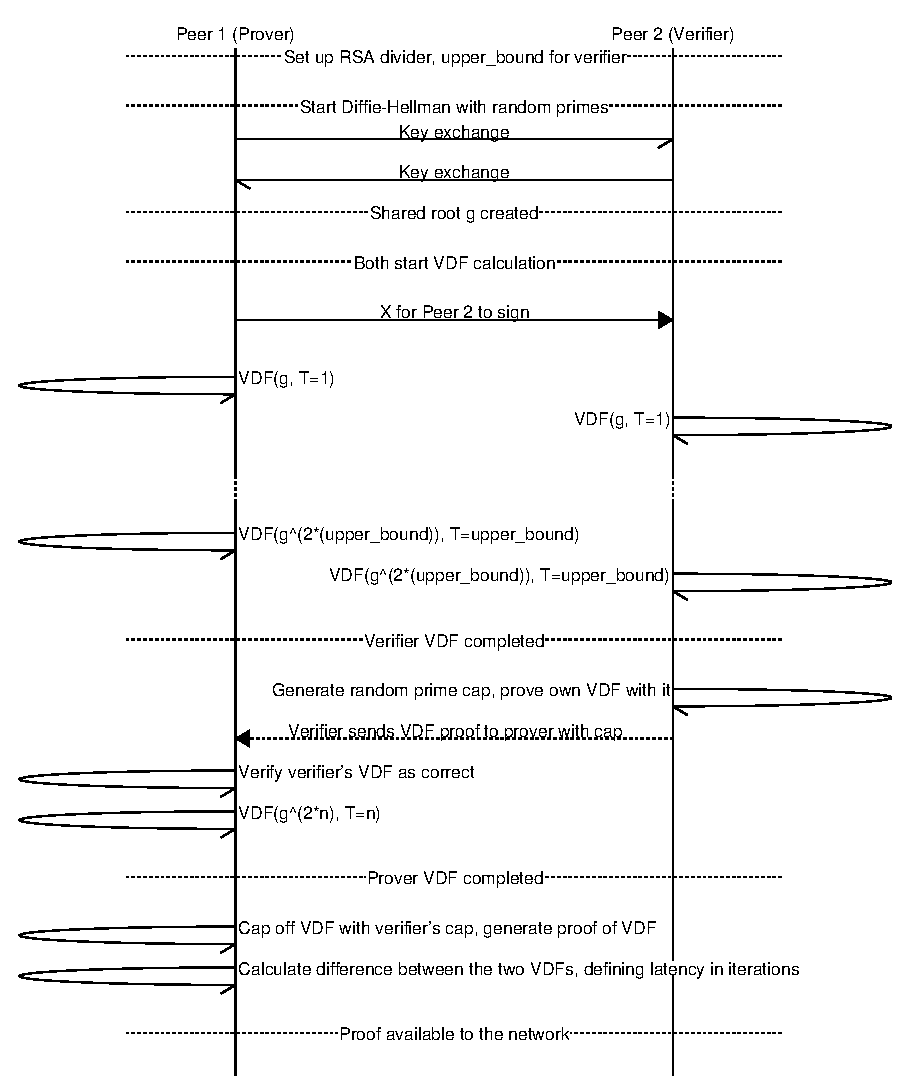
\includegraphics[width=\textwidth]{pictures/pol2_diagram.eps}
	\caption{Protocol Diagram, Proof of Latency}
	\label{PoL Diagram 2}
\end{figure}
Proof of Latency is an interactive public-coin protocol that produces a publicly verifiable non-interactive proof by publishing the parameters with the proof, signed by the participants. The protocol cannot be made non-interactive because of the requirements involved with 
The most important part when calculating any VDF is the setup. If a prover wants to create a valid proof, it needs a previously unknown starting point at first, so that it can prove for certain that it cannot have calculated the VDF in advance. Proof of Latency tackles this problem with a two-way RSA Diffie-Hellman key setup with random ephemeral prime numbers, which is an industry standard to achieve a previously unknown key with large certainty. 

The proof generation removes trust between the two peers by introducing a race between them. The two participants are called the prover and the verifier, although they both are actively proving and verifying their VDFs. The difference here is that they both calculate a VDF and the verifier calculates the difference in iterations between the two.

First the prover and the verifier do a Diffie-Hellman key exchange to construct a previously unknown key. Then, they both start calculating a VDF in parallel. The prover only calculates the VDF up to a predefined threshold, and then sends the proof with a signature back to the verifier. The verifier then stops its own calculation, generates a proof of it, and then calculates the absolute difference between the amount of iterations between its own VDF and the prover's.

Since calculating a VDF is relatively easy for modern processors, a VDF over as little as a few milliseconds of time can be a valid way of measuring latency. Still, without an ASIC chip for calculating VDFs faster than any other available processor, these protocols are also a measurement of processing performance. This might introduce an unfortunate barrier for entry for mobile and IoT devices. The second version of PoL is meant to tackle this problem by creating a performance and latency gradient to the network. The network topology results in a gradient that is defined by geographical location and the similarity in performance. This means that connectedness between mobile and IoT devices is going to be better than between devices that have a huge performance difference.

\section{Attack Vectors}
Since Proof of Latency removes security quarantees by removing randomness from routing, some new attack vectors are introduced. The two versions of the algorithm differ much in terms of security. Proof of Latency is not meant to be a one-stop shop towards a safer network, but rather an add-on to make things more efficient while still keeping security in mind. The following attack vectors are a product of prior knowledge, research and the writer's thought process, and none have been tested out in practice, yet.

\subsection{Advertising Dishonest Peers and Proof Spoofing}
A sybil network participant can spawn an arbitrarily large number of new identities and network peers that are close-by, create multiple Proofs of Latency with them, and only advertise these peers to the rest of the network on their DHT. Two peers can also fake the proof if they co-operate by using VDFs they have already calculated and matched their outputs to be as close as possible. 

This can be mitigated somewhat by requiring peers to renew their proofs regularly, using witnesses or a verifiable source of randomness. Also, trusted computing modules could be used to verify that the software configuration hasn't been changed, removing most of the possibility for side channel attacks against using witnesses.

A way to protect against coordinated proof spoofing is to introduce an unbiased third party to the protocol. Since the soundness of the proof depends largely on the generator and its setup, the proof can be improved by requiring it to be salted by a random input from an unbiased party. How to achieve this? Introduce a salt pool to which a group of PoL witnesses post random salts from which the PoL provers then pick randomly. The witnesses listen for usage of the salts they have generated, and upon receiving the Proof of Latency inspect if their salt has been used or not, and decide to sign or discard the proof based on that.

\subsection{Performance Matching}
Both versions suffer from the same issue, let's call it performance matching, which is a timing attack. Timing attacks are a family of attacks against computer systems called side-channel attacks, which attack the fact that although software is abstract and can be very well fit against any attacks on the software level, outer factors still affect the hardware it runs on. Timing attacks rely on gathering of timing data from the target.~\cite{noauthor_undated-mp} In performance matching, this means connecting to the targeted peer by another protocol or comparing existing proofs of latencies from all peers that have calculated their latency with the target.

Performance matching enables attackers to perform an eclipse attack on low-performance devices by matching the attacker's performance with the targeted mobile device so that it is as close as possible in the difference between iterations in PoL. Now again, if the algorithm had a trusted platform module requirement, or we had an ASIC for repeated squarings, this wouldn't be an issue. This attack could result in a complete network split.

\section{Protecting Against Performance Matching}
\subsection{Hiding Information of VDF Results}
Zero-knowledge proofs could be used to protect against performance matching. If the publicized proof didn't include both the VDF results and iterations, but just included the iteration difference, an attacker would have less info on each peer. This would make attacking more difficult, requiring more queries and PoL runs on average before finding a vulnerable peer.

\subsection{Web of Trust}
There's also a possibility of introducing a web of trust in parallel to PoL to recognize and shut out malicious peers more effectively. An example of such a system is SybilLimit, which adds a construction called trusted routes to DHT based routing.~\cite{Yu2008-xl} I see that trusted routes in conjunction with Proof of Latency would be a great couple. The problem of advertising dishonest peers could also be tackled with a trust based system. Introducing too much trust into the system could also make PoL useless, since there could be a simple ping protocol with a millisecond measurement latency instead.
~
\subsection{Peer Scoring}
Peer scoring is used regularly in P2P networks, 
Proof of Latency serves as a peer scoring metric by itself, and can be used in various ways. To hinder any attacks, peers with the lowest latencies would be kept for a longer time even in the case of the peer not being online, and favoring new ephemeral connections that are farther. 

\subsection{Using a Witness}
A way to make Proof of Latency fully trustless is to introduce an unbiased third party to the protocol. Since the soundness of the proof depends largely on the generator and its setup, the proof can be improved by requiring it to be salted by a random input from an unbiased party. How to achieve this? Introduce a salt pool to which a group of PoL witnesses post random salts from which the PoL provers then pick randomly. The witnesses listen for usage of the salts they have generated, and upon receiving the Proof of Latency inspect if their salt has been used or not, and 

\chapter{Proof of Concept}
\label{Proof of Concept}
To test out Proof of Latency, I made a software proof of concept in Rust. I picked Rust as a programming language because I've wanted to try it out in my own projects for long, and it has some good properties when it comes to cryptography and distributed computing. Since distributed computing or any server program for that matter uses some sort of concurrency to get non-blocking responses to requests they receive, you have a very good chance of running into race conditions with most systems programming languages. When a Rust program has been written in the default "safe" compiler setting, a data race where two or more threads try to access a shared memory resource at the same time is simply impossible to achieve.~\cite{The_Rust_Project_Developers2018-xh} Also, as it is a compiled language without a garbage collector, and with lots of optimization in the compiler, Rust has good baseline performance even when compared to other similarly low level programming languages like Go.~\cite{Howarth2020-zc} Rust has seen a surge of interest in the last few years, and is used in many projects in production, notably in embedded and distributed computing, the former because of Rust's modern build tooling and robustness.

William Borgeaud's blog post~\cite{Borgeaud2019-wk} from November 2019 in particular was the first reference I encountered that described verifiable delay functions in familiar terms to a software engineer like me. The blog post and it's accompanying code~\cite{Borgeaud2019-wk} that also happened to be in Rust helped me bootstrap the project.

First of all, I knew I had to make the VDF run asynchronously, or if possible, in another thread, because it would be one of two VDFs needed in the protocol. There needs to be a separate task for listening to the other party's input, and to make it possible to test locally without networking. For the VDF that is used in Proof of Latency it was also needed that the prover's calculation could be ran indefinitely and ended abruptly by a received "cap" prime number from the verifier. No previous VDF library seemed to have this option, because the difficulty parameter T is usually predetermined in contrast to Proof of Latency.

The code is structured as follows: A runnable binary demo (main.rs) and the reusable library it also uses (lib.rs) resides in the top crate. They both depend on the subcrates "P2P" and "vdf". Here is an example output of Proof of Latency run:
\begin{longlisting}[H]
	\caption{Proof of Latency test run}
	\inputminted
	[
		frame=lines,
		framesep=2mm,
		baselinestretch=1.2,
                breaklines=true,
                fontsize=\footnotesize,
		tabsize=2,
	]
	{text}{./parts/code/samplerun.txt}
	\label{lst:samplerun.txt}
\end{longlisting}

To achieve a better algorithm design, the library itself is described as a state machine, which also helps in thinking of the algorithm in TLA+. Variable names have been converted into more readable non-mathematical forms.
% TODO: Diagram of the state machine, generated by "sm"?

The following is a code example of the threaded evaluation part of a VDF inside proof of latency, containing evaluation stop logic for both the prover and the verifier:
\begin{longlisting}[H]
	\inputminted
	[
		frame=lines,
		framesep=2mm,
		baselinestretch=1.2,
		fontsize=\footnotesize,
		tabsize=2,
	]
	{Rust}{./parts/code/vdfiteration.rs}
        \caption{VDF iteration logic}
	\label{lst:vdfiteration.rs}
\end{longlisting}

The following is a code example of the proof generation of a VDF:
\begin{listing}[H]
	\inputminted
	[
		frame=lines,
		framesep=2mm,
		baselinestretch=1.2,
		fontsize=\footnotesize,
		tabsize=2,
	]
	{Rust}{./parts/code/proofgeneration.rs}
        \caption{VDF proof generation}
	\label{lst:proofgeneration.rs}
\end{listing}

The following is a code example of the verification of a VDF proof:
\begin{listing}[H]
	\inputminted
	[
		frame=lines,
		framesep=2mm,
		baselinestretch=1.2,
		fontsize=\footnotesize,
		tabsize=2,
	]
	{Rust}{./parts/code/verifyvdf.rs}
        \caption{VDF proof verification}
	\label{lst:verifyvdf.rs}
\end{listing}

The proof of concept is made as a library, so that it can be imported in other projects and tinkered with. To make it into a library in addition to a stand-alone binary, I used structs for logical instances of a single VDF, for example. This is mainly to keep program state in instances of these structs, removing possible side effects.

% TODO: TESTS!

\section{Tests}
\subsection{Unit Tests}
To make sure that the VDF calculations worked on arbitrary input by generating a succesfully verifiable proof I made unit tests for the VDF evaluation, proof generation and verification. To further ensure the soundness of the algorithm, I made simulated cases for proof of latency with unit tests with separate, async threads for each execution. Unit tests reside in the same file the program code itself, and the Rust standard library has well enough functionality so that I wasn't forced to use a separate library for assertations\footnote{Checking that a statement holds true or is equal to something}, for example.

In addition to regular unit tests with predefined input, I dabbled in property testing. Property testing is a term that belongs somewhere between fuzzing\footnote{Testing systems against highly randomized and a high volume of input.} and unit tests. Otherwise it functions like regular unit tests, but it adds generated input into the equation. By adding generated, sometimes randomized input, one can check more thoroughly for edge cases. While being effective in recognizing some unexpected bugs, it still has a way to go when compared to formal verification, which is a testing method that aims to define a system with mathematic proofs, verifying that the output should always, apart from hardware issues, be predictable and deterministic.

\subsection{End to End Tests}
To test the whole demo out in a simulated P2P setting I used Protocol Labs' Testground software. It is a tool to simulate a network with thousands of peers on one machine.

\chapter{Future Considerations}
\label{Future Considerations}
If this system was integrated to a blockchain or a publicly verifiable source of randomness for the initial setup, the proofs could be verified by anyone against consensus. Not only this would add trust to the latency measurements, but also speed up initial bootstrapping of the P2P network. When P2P networks eventually grow larger and larger, the network bootstrapping infrastructure needs to be rethought to handle more traffic and be faster in its initialization. By getting introduced to the closest peers possible right at the start the user can experience a more performant network right from the beginning, lowering the barrier for entry by making first impressions better. 

Also, I believe the work is not cryptographically as secure as it could be, and the field is progressing at a mindnumbing pace. Making sure the algorithm is VDF-agnostic would be a logical next step, since the field is still in progress of finding the best possible formulation of a VDF. Quantum computing can render all existing VDF types insufficient, and new VDF types could change the parameter logic fundamentally. The idea behind this thesis is to think of a new creative way of using verifiable delay functions by defining a protocol, and not to necessarily use the most robust cryptography available. 


\chapter{Conclusion}
\label{Conclusion}
Since calculating a VDF is relatively easy for modern processors, a VDF over as little as a few milliseconds of time can be a valid way of measuring latency. Still, without an ASIC chip for calculating VDFs faster than any other available processor, Proof of Latency is also a measurement of processing performance. This might introduce an unfortunate barrier for entry for mobile and IoT devices. When used in P2P routing optimization, PoL will result in a network topology organized by a gradient that is defined by geographical location, network connection speed and the similarity in performance between peers.

This means closely located and similarly performant devices form strong local topologies that are bridged by their random connections to other peers and also by the connections they have to performant local peers. Highly performant devices form strong connections with each other whether they are located near each other or not, because other devices cannot compete against them in the race that is Proof of Latency, resulting in a network topology that is locally effective but global at the same time. The reality that VDFs can't be sped up by additional processors or cores means that the gradient will not be as drastic as one might imagine.

Proof of Latency as a peer scoring metric not only protects peers from eclipse attacks, but can also function as a way of speeding up the initial bootstrapping process by bringing peers more closely together. This also makes the resulting P2P network more robust, due to its locality, in instances of internet stoppages between continents, censorship, or high network load. When used to prove a geographical location, Proof of Latency can combat fraud in applications that rely on GPS location.

\section{Future Considerations}
If this system was integrated to a blockchain or a publicly verifiable source of randomness for the initial setup, the proofs could be verified by anyone against consensus. Not only this would add trust to the latency measurements, but also speed up initial bootstrapping of the P2P network. When P2P networks eventually grow larger and larger, the network bootstrapping logic needs to be rethought to handle more traffic, be more decentralized, and be faster in its initialization. By getting introduced to the closest peers possible right at the start the user can experience a more performant network faster, lowering the barrier for entry and making first impressions better.

Also, I believe the work is not cryptographically as secure as it could be, and the field is progressing at a mindnumbing pace. Making sure the algorithm is VDF-agnostic would be a logical next step, since the field is still in progress of finding the best possible formulation of a VDF. Quantum computing can, or will, render all existing VDF types insufficient, and new VDF types could change the parameter logic fundamentally.


% insert references
%  - included unsrtf.bst provides finnish language version of unsrt
\bibliographystyle{unsrt}
\bibliography{library.bib}

%%%%%%%%%%%%%%%%%%%%%%%%%%%%%%%%%%%%%%%%%%%%%%%%%%%%%%%%%%%%%%%%%%%%%%%%%%%
%
% Almost there....
%
%%%%%%%%%%%%%%%%%%%%%%%%%%%%%%%%%%%%%%%%%%%%%%%%%%%%%%%%%%%%%%%%%%%%%%%%%%%

% make sure pagecount is correct even if references overflow to a new page
\pagebreak\addtocounter{page}{-1}
\eofpages
\appendices

% create your appendix chapters with command \appchapter{some name} instead
% of \chapter{some name} for the automagic page counting to work
%\input{file name of appchapter xxx}
%\input{file name of appchapter yyy}
%\input{file name of appchapter zzz}
%\input{and so on}

%%%%%%%%%%%%%%%%%%%%%%%%%%%%%%%%%%%%%%%%%%%%%%%%%%%%%%%%%%%%%%%%%%%%%%%%%%%
%
% main document ends here
%
%%%%%%%%%%%%%%%%%%%%%%%%%%%%%%%%%%%%%%%%%%%%%%%%%%%%%%%%%%%%%%%%%%%%%%%%%%%
\eofapppages
\end{document}
